\documentclass{article}
\usepackage{url,amsfonts, amsmath, amssymb, amsthm, graphicx, braket, fancyhdr, physics, mathtools, hyperref}
% Change this path if you use images
\graphicspath{ {./Classical_Images/} }
% Page layout
\setlength{\textheight}{8.75in}
\setlength{\columnsep}{2.0pc}
\setlength{\textwidth}{6.5in}
\setlength{\topmargin}{0in}
\setlength{\headheight}{0.0in}
\setlength{\headsep}{0.0in}
\setlength{\oddsidemargin}{0in}
\setlength{\evensidemargin}{0in}
\setlength{\parindent}{1pc}

% Commands
\newcommand{\RNum}[1]{\uppercase\expandafter{\romannumeral #1\relax}}
\newcommand{\Lagr}{\mathcal{L}} % Lagrangian
\newcommand{\vcurl}[1]{\vec{\nabla}\times \vec{#1}}

\usepackage[a4paper,margin=2.5cm,portrait, headsep=24pt, headheight=2cm]{geometry}
\usepackage{enumitem}

% Header
\pagestyle{fancy}
\fancyhf{}
\rhead{Page \thepage}
\chead{Classical Mechanics DE}
\lhead{James Natoli}
\rfoot{}

\begin{document}
% suppress header on first page
\thispagestyle{empty}
%%% Title Stuff
\begin{center}\Large \textbf{Classical Mechanics Departmental Exam} \\
\normalsize James Natoli \\  January 2021
\end{center}

%%%%%%%%%%%%%%%%% Problem 1 %%%%%%%%%%%%%%%%%
\section*{Problem 1} 
% Problem Statement
Consider a planet in a circular orbit around a star. Determine how the speed of the planet depends on how far away it is from the star. Does Pluto move faster or slower than Mercury around the run?
%% Solution Here
\section*{\textit{Solution}} 
Let's start with centripetal force, $ F_c = \frac{mv^2}{r}$ and gravitational force, $F_g = G\frac{Mm}{r^2}$
As these are the only forces, we can set them equal to each other and work from there
\begin{align}
\frac{mv^2}{r} &= G\frac{Mm}{r^2} \\
v^2 &= \frac{GM}{r} \\
v &= \sqrt{\frac{GM}{r}} \\
v &\propto \frac{1}{\sqrt{r}} 
\end{align}
So because velocity depends on $ \frac{1}{\sqrt{r}}$, \boxed{\text{Pluto will move slower than Mercury}}
%%%%%%%%%%%%%%%%% Problem 2 %%%%%%%%%%%%%%%%%
\section*{Problem 2} 
% Problem Statement
A satellite in circular orbit of radius R about the center of the earth is subject to a drag force of magnitude $F = av^n$ (where $v$ is the speed of the satellite) which results in the rate of change of the radial distance $\frac{dr}{dt} = -b$ (where $b > 0$ is small enough so that the loss of energy in an orbit is small compared to the total kinetic energy of the satellite). Determine $a$ and $n$
%% Solution Here
\section*{\textit{Solution}} 
Start with the Virial Theorem, which states that the average kinetic energy is equal to minus one half of the average potential energy, or
\[ T_{avg} = -\frac{1}{2}V_{avg} \]
In circular orbits, $ T_{avg} =T$ and $V_{avg} = V$
\begin{align}
	E = T + V &= -\frac{1}{2}V + V = \frac{1}{2}V \\ 
	\text{where gravitational potential is }V &= -\frac{GMm}{r} \\ 
	E &= -\frac{GMm}{2r} 
\end{align}
Next, we have to find a way to get some derivatives, because the problem gives us $\frac{dr}{dt} = -b$
\begin{align}
	dW = E &= \vec{F} \cdot \vec{x} \\
	\frac{dE}{dt} &= \vec{F} \cdot \frac{d\vec{x}}{dt} \\  
	\frac{dE}{dt} &= \vec{F} \cdot \vec{v} \\ 
	\text{and using (7), }& \\
	\frac{dE}{dt} &= \frac{GMm}{2r^2} \dot{r} \\ 
	\text{now use }& \dot{r} = -b, \\ 
	\frac{dE}{dt} &= -\frac{GMm}{2r^2} b
\end{align}
We also know that $\vec{F} \cdot \vec{v} = -av^n \cdot v = -av^{n+1}$, where this is negative because drag force is always opposite the direction of motion
Also recall from circular orbits (or the previous problem) that when we set centripetal force = gravitational force, we get $v = \sqrt{\frac{GM}{r}}$, so this leaves us with
\[ \vec{F} \cdot \vec{v} = -a\left(\frac{Gm}{r}\right)^\frac{n+1}{2} \]
Now use this (above) combined with (10) and (7) to get
\[ -\frac{GMm}{2r^2}b = -a\left(\frac{Gm}{r}\right)^\frac{n+1}{2} \]
To find a and n, we can set $n = 1$
\[ \frac{GMm}{2r^2}b = a\frac{GM}{r} \]
\[\boxed{a = \frac{mb}{2r}} \]
I suppose you could find $a$ for other values or $n$, or solve them for each other, but this was about as far as I felt like going 

%%%%%%%%%%%%%%%%% Problem 3 %%%%%%%%%%%%%%%%%
\section*{Problem 3 } 
% Problem Statement
Consider a mass m in a circular orbit of radius R in a central-force potential $-am/r^n,a>0$. Determine the range of $n>0$ for which such a circular orbit is stable
%% Solution Here
\section*{\textit{Solution}} 
Alrighty, let's first recall the condition for stability. As far as mental stability goes, I'm in the dark, but for orbital stability we require that the second spatial derivative of the effective potential is $>$ 0
\[ \frac{d^2V_{eff}}{dr^2} > 0\]
where the effective potential is, $V_{eff} = V + \frac{l^2}{2mr^2}$
\begin{align}
	\frac{dV_{eff}}{dr} = \frac{d}{dr}\left(\frac{l^2}{2mr^2} - \frac{am}{r^n}\right) &= 0 \\ 
	= -\frac{l^2}{mr^3} + \frac{anm}{r^{n+1}} &= 0 \\ 
	\frac{l^2}{mr^3} &= \frac{anm}{r^{n+1}} \\ 
	\frac{d^2V_{eff}}{d^2r} = \frac{d}{dr}\left( -\frac{l^2}{mr^3} + \frac{anm}{r^{n+1}}\right) &> 0 \\
	\frac{3l^2}{mr^4} - \frac{(n+1)nam}{r^{n+2}} &> 0 \\ 
	\frac{3}{r} \left(\frac{l^2}{mr^3}\right) - \frac{(n+1)nam}{r^{n+2}} &> 0 \\
	\text{now we use (17), } \frac{3}{r} \left(\frac{nam}{r^{n+1}}\right) - \frac{(n+1)nam}{r^{n+2}} &> 0 \\
	3 \left(\frac{nam}{r^{n+2}}\right) - (n+1) \left( \frac{nam}{r^{n+2}} \right) &> 0 \\
	3 - (n+1) &> 0 \\
	2 &> n
\end{align}
And so, \boxed{n < 2} in order for the orbit to be stable \\
\\
Note: I'm not exactly sure why we set the original first derivative to 0, maybe because we're looking at the potential minimum

%%%%%%%%%%%%%%%%% Problem 4 %%%%%%%%%%%%%%%%%
\section*{Problem 4} 
% Problem Statement
The gravitational acceleration on the surface of the moon is one-sixth of that on the surface of the earth. A woman on Earth lowers her center of mass by 40 cm by bending her knees. Exerting a constant force on the ground, she jumps straight up, raising her center of mass by 60 cm above that of her normal erect position. How much higher can she jump on the moon?
%% Solution Here
\section*{\textit{Solution}} 
First, let's establish that $\Delta h_{earth} = 1.0$ m. She also applies the same force both times, over the same distance, so we can also say that $W_{Earth} = W_{Moon}$
\begin{align}
	W_{Earth} &= V_{final} - V_{initial} \\
	&= mgh_f - mgh_i \\ 
	&= mg(\Delta h_{earth})
\end{align}
We also have the following expression for the moon's work
\[ W_{Moon} = m \left( \frac{g}{6} \right) \Delta h_{Moon} \]
Now, let's set these 2 work expressions equal to eachother...
\begin{align}
	W_{Moon} &= W_{earth} \\ 
	m \left( \frac{g}{6} \right) \Delta h_{Moon} &= mg(\Delta h_{earth}) \\
	\Delta h_{Moon} &= 6 \Delta h_{earth}
\end{align}
So she can jump \boxed{\text{ six times higher}} than on Earth

%%%%%%%%%%%%%%%%% Problem 5 %%%%%%%%%%%%%%%%%
\section*{Problem 5} 
% Problem Statement
A uniform rigid rod of length L, mass m, and moment of inertia $mL^2/3$ about an end, is supported horizontally by props at each end. Find the force at the second prop right after the first one is removed.
%% Solution Here
\section*{\textit{Solution}} 
This problem was a little difficult for me to visualize, so I've included a picture
\begin{figure}[h]
	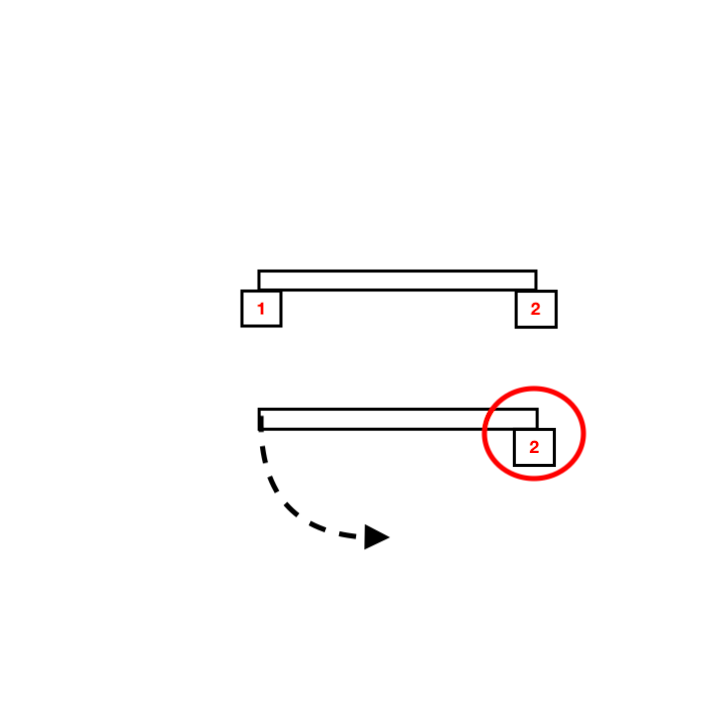
\includegraphics[scale=0.5]{P5}
	\centering
\end{figure}
Here, we can see the support on the left has been removed, allowing the rod to swing down. We are focusing on the force on the support on the right the moment it is removed. Let's start with a free-body diagram. In lieu of drawing it, we can see that there are only 2 forces involved, gravity pulling the bar down and acting on its center of mass, and the force from the support, pushing back up. 
\[ \Sigma F_y = mg - F_s = ma_y \]
Where $a_y$ is acceleration in the y direction and $F_s$ is the support force, what we are solving for
\[ F_s = mg - ma_y \]
We also need to consider Torques, because the gravitational force is acting at the center of mass, not the point of rotation. Lets state the same law but for Torques
\begin{align}
	\Sigma \tau = I \ddot{\theta} &= \vec{r} \times \vec{F_g} \\
	\frac{mL^2}{3} \ddot{\theta} &= \frac{L}{2} \cdot mg \\
	\ddot{\theta} &= \frac{3g}{2L}
\end{align}
In (29) the cross product simplifies to multiplication because the radial vector is perpendicular to $F_g$, and $r = \frac{L}{2}$ because that is the distance to the center of mass, the midpoint of the rod \\ \\ 

Now, we use some angular to linear conversions, listed below
\begin{align}
	v_y &= r\dot{\theta} \\
	a_y &= r\ddot{\theta} \\
	r &= \frac{L}{2}
\end{align}

Now let's put (32) - (34) together with $ F_s = mg - ma_y $ and solve

\begin{align}
	F_s &= mg - ma_y \\ 
	&= mg - m\left( \frac{L}{2} \right) \left( \frac{3g}{2L} \right) \\
	&= mg - \frac{3mg}{4} \\ 
	&= \frac{mg}{4}
\end{align}
And so \boxed{F_s = \frac{mg}{4}} at the moment the first support is released

%%%%%%%%%%%%%%%%% Problem 6 %%%%%%%%%%%%%%%%%
\section*{Problem 6} 
% Problem Statement
Consider two identical masses m and two identical springs of spring constant k and unstretched length a.
\begin{figure}[h]
	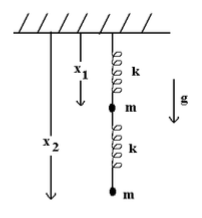
\includegraphics[scale=0.5]{P6}
	\centering
\end{figure}
\begin{enumerate}[label=\alph*)]
	\item % PART (A)
	What are the equilibrium positions $x_{10}$ and $x_{20}$?
	\item % PART (B)
	For small vertical oscillations about  $x_{10}$ and $x_{20}$ what are the normal frequencies?
	\item % PART (C)
	What are the motions associated with each of these frequencies?
\end{enumerate}
%% Solution Here
\section*{\textit{Solution}} 
\begin{enumerate}[label=\alph*)]
	\item % PART (A)
	Let's look first at the top spring
	\[ \Sigma F_y = F_g + F_s = 0 \text{ bc at equilibrium} \]
	Here we have our familiar spring force $F_s = k\Delta x$, where $\Delta x = x_{10} - a$, basically just the unstretched length, plus the equilibrium position from gravity pulling the spring down slightly. We also have $F_g = 2mg$, where this is accounting for the bottom mass pulling down on the top mass. This leaves us with
	\[ 2mg = k(x_{10} - a) \]
	\[ \boxed{x_{10} = \frac{2mg}{k} + a }\]
	And let's repeat this for the bottom spring, but using $\Delta x = x_{20} - x_{10} - a$ and $F_g = mg$
	\[ mg = k(x_{20} - x_{10} - a) \]
	\[ x_{20} = \frac{mg}{k} + x_{10} + a \]
	\[ \boxed{x_{20} = \frac{3mg}{k} + a }\]
	\item % PART (B)
	Ok, now we're actually gonna do some real classical mechanics. Basic Process will be 1) getting Lagrangian then 2) Using Euler-Lagrange equations
	\begin{align}
		\Lagr &= T - V \\ 
		\Lagr &= \frac{1}{2}m\left(\dot{x_1}^2 + \dot{x_2}^2\right) + mg\left(x_1 + x_2\right) - \frac{1}{2}k\left[(x_1 - a)^2 + (x_2 - x_1 - a)^2\right] \\ 
	\end{align}
	Keep an eye on the signs here, especially on gravitational potential and spring potential terms. Ok, next lets take our derivatives, recalling the standard Euler-Lagrange equations for functions of position and time
	\begin{align}
		&\dv{}{t} \left( \pdv{ \Lagr}{\dot{x_i}} \right) = \pdv{\Lagr}{x_i} \\
		\pdv{ \Lagr}{\dot{x_1}} &= mg - \frac{1}{2}k\left[2(x_1 - a) - 2(x_2 - x_1 -a) \right] \\
		&= mg - \frac{1}{2}k\left[2x_1 - 2a - 2x_2 + 2x_1 + 2a \right] \\
		&= mg - \frac{1}{2}k\left[4x_1 - 2x_2\right] \\
		&= mg - k\left[2x_1 - x_2\right] \\
		\pdv{ \Lagr}{\dot{x_2}} &= mg - \frac{1}{2}k\left[ 2(x_2 - x_1 -a) \right] \\
		&= mg - k\left[x_1 - x_1 - a\right]
	\end{align}
	The time derivatives are a little easier, so lets do those next
	\begin{align}
		\dv{}{t} \left( \pdv{ \Lagr}{\dot{x_1}} \right) = m\ddot{x_1}, &\hspace{1cm} \dv{}{t} \left( \pdv{ \Lagr}{\dot{x_2}} \right) = m\ddot{x_2} \\
		\text{ now using (44) to combine (48)}&\text{ and (51)} \\ 
		\Longrightarrow \ddot{x_1} &= g - \frac{k}{m}(2x_1 - x_2) \\
		\text{ and using (44) to combine (50)}&\text{ and (51)} \\ 
		\Longrightarrow \ddot{x_2} &= g - \frac{k}{m}(x_2 - x_1 - a)
	\end{align}
	There's still more work to do, sadly, as we must consider small oscillations. These will take the form of 
	\[ x_1 = x_{10} + \Delta x_1 \hspace{1cm}\text{ and} \hspace{1cm} x_2 = x_{20} + \Delta x_2 \]
	\begin{align}
		\Delta\ddot{x_1} &= g - \frac{k}{m}(2x_{10} + 2\Delta x_1 - x_{20} - \Delta x_2) \\
		\intertext{now use the boxed results from (A) for the equilibrium positions, $x_{10}$  and $x_{20}$}
		\Delta\ddot{x_1} &= g - \frac{k}{m}\left(\frac{4mg}{k} + 2a + 2\Delta x_1 - \frac{3mg}{k} - 2a - \Delta x_2\right) \\
		\Delta\ddot{x_1} &= g - 4g - \frac{2k}{m}\Delta x_1 + 3g + \frac{k}{m} \Delta x_2 \\
		\Delta\ddot{x_1} &= \frac{k}{m}(\Delta x_2 - 2\Delta x_1) \\ 
		\intertext{and for the 2nd mass}
		\Delta\ddot{x_2} &= g - \frac{k}{m}(2x_{20} + 2\Delta x_2 - x_{10} - \Delta x_1 - a) \\
		\Delta\ddot{x_2} &= g - \frac{k}{m}\left(\frac{3mg}{k} + 2a + 2\Delta x_2 - \frac{2mg}{k} - a - \Delta x_1 - a\right) \\
		\Delta\ddot{x_2} &= g - 3g - \frac{k}{m}\Delta x_2 + 2g + \frac{k}{m} \Delta x_2 \\
		\Delta\ddot{x_2} &= \frac{k}{m}(\Delta x_1 - \Delta x_2)
	\end{align}
	Alrighty, as if that wasn't enough, we now can approximate those small oscillations as follows
	\[ \Delta x_1 = Ae^{i\omega t} \hspace{1cm} \text{ and } \hspace{1cm} \Delta x_2 = Be^{i\omega t} \]
	Thereby giving us the following second derivatives
	\[ \Delta x_1 = -A\omega^2e^{i\omega t} \hspace{1cm} \text{ and } \hspace{1cm} \Delta x_2 = -B\omega^2e^{i\omega t} \]
	We're now going to set up a lil system of equations, and do some fun matrix eigenvalue analysis on it. Let's rearrange (60) and (65) as
	\begin{align}
		\Delta\ddot{x_1} - \frac{k}{m}(\Delta x_2 - 2\Delta x_1) &= 0 \\ 
		\Delta\ddot{x_2} - \frac{k}{m}(\Delta x_1 - \Delta x_2) &= 0 \\
		\intertext{now plug in the exponential approximations}  
		-A\omega^2e^{i\omega t} - \frac{k}{m}(Be^{i\omega t}- 2Ae^{i\omega t}) &= 0 \\
		-B\omega^2e^{i\omega t} - \frac{k}{m}(Ae^{i\omega t}- Be^{i\omega t}) &= 0 \\
		\intertext{and now we can divide out the exponential factor} 
		A \left( \frac{2k}{m} - \omega^2 \right) + B \left( \frac{-k}{m} \right) &= 0 \\
		A\left( \frac{-k}{m} \right)  + B \left( \frac{k}{m} - \omega^2 \right) &= 0 
	\end{align}
	This is now in a handy dandy form that we can grab some pretty eigenvalues from, so lets make our eigenvalue equation
	\[\begin{pmatrix} \frac{2k}{m} - \omega^2 & \frac{-k}{m} \\ \frac{-k}{m} & \frac{k}{m} - \omega^2 \end{pmatrix} 
	\begin{pmatrix} A \\ B \end{pmatrix} = 0\]
	Matrices scare me, so I'm gonna do this the way I know how, let's set the determinate of the 2x2 matrix = 0 and then solve
	\begin{align}
		\left( \frac{2k}{m} - \omega^2 \right) \left( \frac{k}{m} - \omega^2 \right) - \left( \frac{-k}{m} \right)\left( \frac{-k}{m} \right) &= 0 \\ 
		\omega^4 - \frac{3k}{m}\omega^2 + \frac{2k^2}{m^2} - \frac{k^2}{m^2} &= \omega^4 - \frac{3k}{m}\omega^2 + \frac{k^2}{m^2} \\ 
		\intertext{sauce some quadratic ketchup on this bad boy and see what kinda fry we have} 
		\omega^2  = \frac{ \frac{3k}{m} \pm \sqrt{ \frac{9k^2}{m^2} - \frac{4k^2}{m^2}}}{2} &= \frac{ \frac{3k}{m} \pm \frac{k}{m}\sqrt{5}}{2}
		\intertext{here we can see due to the plus/minus we have two distinct modes}
		\boxed{ \omega_+^2 = \frac{k}{m} \left( \frac{3 +\sqrt{5}}{2} \right) \text{ and } \omega_-^2 = \frac{k}{m} \left( \frac{3 -\sqrt{5}}{2} \right) }
	\end{align}
	\item % PART (C)
	All that's left now is to describe the motions that are associated with these 2 frequencies. Basically, we can either symmetric or antisymmetric motion, which is determined by the relative signs of A and B. \\ 
	\[ \omega_+^2 \Longrightarrow \text{ A, B have opposite signs $\Longrightarrow$ Antisymmetric Motion} \]
	\[ \omega_-^2 \Longrightarrow \text{ A, B have the same signs $\Longrightarrow$ Symmetric Motion} \]
	For the positive sign, I picture the two masses bouncing against each other, always traveling in the opposite direction as the other. On the other hand for the negative sign, I picture the masses moving together \\
	\\ 
	Extra Resources: \\ 
	\url{http://electron6.phys.utk.edu/PhysicsProblems/Mechanics/6-Oscillations/coupled-spring.html} \\ 
	\url{http://sites.science.oregonstate.edu/~gibsonn/Teaching/MTH323-010S15/Supplements/coupled_spring.pdf}
\end{enumerate}

%%%%%%%%%%%%%%%%% Problem 7 %%%%%%%%%%%%%%%%%
\section*{Problem 7} 
% Problem Statement
Over a day, meteors deposit on the surface of the Earth a uniform layer of dust of thickness $\Delta R$, small compared to the radius of the Earth $R$. If $\rho_{dust}$ and $\rho_{earth}$ are the densities of dust and the Earth, show that conservation of angular momentum results in the change of the length of the day by approximate $5\Delta R \rho_{dust} / (R \rho_{earth})$. The moment of inertia of a sphere of mass M and radius R about a central axis is $2MR^2/5$, and that of a thin spherical shell of mass M and radius R is $2MR^2/3$ about a central axis.
%% Solution Here
\section*{\textit{Solution}} 
What a weird problem. Basically what it's saying is that because the radius of the earth increases ~slightly~ due to the meteor dust, then the earth must slow down its rotation in order to conserve angular momentum. In an extreme example, think of the classic ice skater moving their arms outward (thereby increasing the radius of rotation) and slowing down. \\
The reason we're given that second moment of inertia is because we're going to treat the dust as a super thin shell that's covering the earth. Ok, enough jabbering from me, let's dive in to the angular momentum pond with some conservation statements
\begin{align}
	l_i = I_e\omega_i &\text{ for initial and } l_f = I_e\omega_f + I_d\omega_f \text{ for final} \\
	\intertext{conservation of angular momentum says that these need to be equal, so let's make it so!} 
	I_e\omega_i &= I_e\omega_f + I_d\omega_f \\ 
	\frac{\omega_i}{ \omega_f} &= 1 + \frac{I_d}{I_e} \\ 
	&= 1 + \left( \frac{ \frac{2}{3} M_d \Delta R^2}{\frac{2}{5}M_e R^2} \right)
\end{align}
Uhhh ok so this was good, but it will actually be more helpful to use T = period = $\frac{2\pi}{\omega}$, rather than angular velocity $(\omega)$
\begin{align}
	I_i\left( \frac{2\pi}{T_i} \right) &= I_f\left( \frac{2\pi}{T_f} \right) \\ 
	T_f &= \frac{I_f}{I_i}T_i \\
	T_f &= \left( \frac{I_e + I_d}{I_e} \right) T_i \\
	\intertext{we want the change in length of the day, so looking for the difference between initial and final} 
	T_f &= T_i + \left( \frac{I_d}{I_e} \right) T_i \\ 
	T_f - T_i &= \left( \frac{I_d}{I_e} \right) T_i \\ 
	\intertext{let's say we want the percent change, then we'll look for the following}
	\% \hspace{0.1cm} change &= \frac{T_f - T_i}{T_i} \\
	&= \frac{I_d}{I_e} \\ 
	&=  \frac{ \frac{2}{3} M_d \Delta R^2}{\frac{2}{5}M_e R^2}
	\intertext{Unfortunately, we don't have the mass of dust or earth, but we were given volume, so we can take advantage of the relationship between density, mass, and volume}
	M_{earth} &= \frac{4}{3} \pi R^3 \cdot \rho_{earth} \\
	V_{dust} &\approx \text{Surface Area} \times \text{Thickness} \\ 
	V_{dust} &\approx 4\pi R^2 \Delta R \\ 
	M_{dust} &\approx 4\pi R^2 \Delta R \cdot \rho_{dust}
	\intertext{Now, we'll use (85) to combine (86) and (89)}
	\frac{\Delta T}{ T_i} &\approx \frac{ \frac{2}{3} \left(4\pi R^2 \Delta R \rho_d \right) R^2}
		{\frac{2}{5} \left( \frac{4}{3} \pi R^3 \rho_e \right) R^2} \\ 
	&\boxed{ \frac{\Delta T}{ T_i} \approx \frac{5 \Delta R \rho_d}{R \rho_e} }
\end{align}
As was to be proven. If that little bit about the volume of the dust is confusing, I imagined it like a bunch of sheets of paper stacked on top of each other. To find the volume of the stack, you'd take the area of one sheet and multiply it by the thickness of the stack.

%%%%%%%%%%%%%%%%% Problem 8 %%%%%%%%%%%%%%%%%
\section*{Problem 8} 
% Problem Statement
The free surface of a liquid is an isopotential surface. By considering the potential energy density of an incomprehensible liquid in a vessel rotating about a vertical axis at a constant angular velocity $\omega$, show that the free liquid surface is a paraboloid of revolution
%% Solution Here
\section*{\textit{Solution}} 
Straight out of candyland with this question, literally don't think I've ever once answered a question about liquids in a physics class. Anyways, someone smarter than me had the Lagrangian laid out, so we can just start there and hit it with our Euler-Lagrange equations. 
\[ \Lagr = T - V = \frac{1}{2}m\dot{r}^2 + \frac{1}{2}m\dot{r}^2\omega^2 - mgz(r) \]
Ok so let's walk through this Lagrangian and try to understand. 
\begin{itemize}
\item First term ($\frac{1}{2}m\dot{r}^2$) is your standard Kinetic Energy, where $\dot{r}$ is our radial velocity, or how fast are the particles changing their distance from the center. 
\item Second term ($\frac{1}{2}m\dot{r}^2\omega^2$) is another Kinetic Energy term, but this time for the angular motion. This is their energy as they move around the axis of rotation.
\item Third term ($mgz(r)$) must therefore be our potential, which is essential the height of the liquid. As the liquid rotates, it will ride up the side of the vessel, thereby increasing gravitational energy. 
\end{itemize}
The variable $z(r)$ will be the height of the liquid at a certain distance, r, from the center of rotation. When the question asks "show that the free liquid surface is a paraboloid of revolution", what it really wants us to do is show that $z(r)$ is parabolic, or that $z(r) \propto r^2$
\begin{align}
	\intertext{Let's start with reminding ourselves what the Euler-Lagrange equations are}
	\dv{}{t} \left( \pdv{ \Lagr}{\dot{x_i}} \right) &= \pdv{\Lagr}{x_i} \\
	\dv{}{t} \left( \pdv{ \Lagr}{\dot{r}} \right) &= \pdv{\Lagr}{r} \\ 
	m\ddot{r} &= mr\omega^2 - mg \dv{z}{r} \\
	(\ddot{r} - r\omega^2)dr &= -gdz \\
	\intertext{We now make the seemingly random assumption that $\dot{r} = 0$, because water is well behaved. This probably relates to the incompressibility, if the water is traveling outwards/inwards, it has nowhere to go. Angular velocity is ok, because the motion is a continuous circle}
	r\omega^2dr &= -gdz  \\
	\int r\omega^2dr &= -\int gdz \\ 
	\frac{r^2\omega^2}{2} &= gz(r) + c \\
	\Aboxed{z(r) &= \frac{r^2\omega^2}{2} + c}
\end{align}
This is a paraboloid, as was to be proven
%%%%%%%%%%%%%%%%% Problem 9 %%%%%%%%%%%%%%%%%
\section*{Problem 9} 
% Problem Statement
Two graduate students, each of mass $m_g$, stand at one end of a long flat car of mass $m_c$ that has frictionless wheels. Either student can run to the other end of the cart and jump off with speed u (relative to the cart).
\begin{enumerate}[label=\alph*)]
	\item % PART (A)
	Find the recoil speed of the cart if both students run and jump off simultaneously.
	\item % PART (B)
	What is the recoil speed of the cart if the second student starts running only after the first has jumped off? Is this less than or greater than that in (a)?
\end{enumerate}
%% Solution Here
\section*{\textit{Solution}}
I do believe there a few ways to solve this one, so if I am annoying check some other solutions
\begin{enumerate}[label=\alph*)]
	\item % PART (A)
	For this, all we really need is conservation of momentum
	\begin{align}
		p_i &= p_f \\
		m_i v_i &= m_c v + 2mg(u + v)
		\intertext{Here v is the final velocity of the cart, that's why the two students travel at $u+v$, the carts speed plus their speed relative to the cart (can be forwards or backwards, whichever makes more sense to you). We also set $v_i = 0$ because the initial velocity won't matter and so zero is easier}
		0 &= m_c v + 2mgu + 2mgv \\ 
		\Aboxed{v &= \frac{-2m_g u}{m_c + 2m_g} }
		\intertext{Looking at this, the signs make sense, because if $u >0$ (that is, the students jump off the front) they'll push the cart back, and its velocity will be negative. However if $u<0$ (that is, the students jump off the back) they'll push the cart forwards, and its velocity will be positive}
	\end{align}
	\item % PART (B)
	This is where the fun begins. I'll work through the math first, and then jabber a little afterwards
	\begin{align}
		\intertext{For the first jump, conservation of energy states that}
		0 &= (m_c + m_g)v_1+ m_g(u + v_1)
		\intertext{Where here $v_1$ is the speed of the cart (and remaining student) after the first jump}
		-m_gu &= (m_c + 2m_g)v_1 \\ 
		v_1 &= \frac{-m_gu}{m_c + 2m_g}
		\intertext{And now the second student yeets off, so we do have an initial momentum}
		(m_c + m_g)v_1 &= m_c v_2 + m_g(u + v_2) \\ 
		(m_c + m_g)v_1 - m_g u &= (m_c + m_g)v_2 \\
		v_2 &= v_1 - m_g u \\ 
		\Aboxed{v_2 &= \left( \frac{-m_g u}{m_c + 2m_g} \right) - \left( \frac{m_g u}{m_c + m_g} \right)}
	\end{align}
	It is clear from this that $v_2 < v$ from part (A), because we are subtracting an additional term, so the recoil speed is actually lower if they jump off separately. This is because when the first person jumps by themselves, they must push against the cart \underline{as well as} the remaining student, whereas when they jump together, they are combining their forces to push against the cart. Another more extreme example of this, is to imagine a train car full of sand. If the sand is allowed to release slowly (essentially one at a time, like part (B)), the car will not move. However, if all of the sand is dumped at once, the car will almost certainly move in the opposite direction. One grain of sand acting on its own is negligible, only when they act as a UNION, can they achieve something great. 
\\ 
\\
If you're bored, watch \href{https://www.youtube.com/watch?v=j5b6fpSkqAE}{this video} and imagine them being unloaded one-by-one, versus all at once (skip to like :37)
\end{enumerate}

%%%%%%%%%%%%%%%%% Problem 10 %%%%%%%%%%%%%%%%%
\section*{Problem 10} 
% Problem Statement
A uniform thin semicircular sheet of metal (of radius R) lies in the xy plan with its center at the origin and diameter lying along the x axis. Find the position of the center of mass.
%% Solution Here
\section*{\textit{Solution}} 
\begin{figure}[h]
	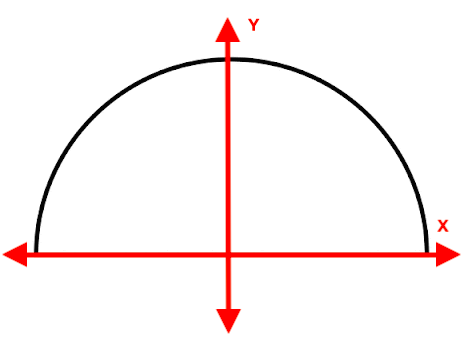
\includegraphics[scale=0.35]{P10}
	\centering
\end{figure}
Our dear, deer old friend center of mass integral has once again returned to haunt us. As can be seen from the diagram, I've oriented the semicircle such that it is symmetric about the y-axis, giving
\[ \boxed{ X_{COM} = 0} \]
To find the $Y_{COM}$, we will have to integrate. Let's recall the integral formula for Center of Mass
\begin{align}
	Y_{COM} &= \frac{ \int \rho y da}{\int \rho da} \\ 
	\intertext{Here $\rho$ is the density, it's uniform though so don't worry, it comes out of the integral and divides out. We'll also use $y = r\sin{\theta}$}
	&= \frac{ \int_0^R \int_0^{\pi} (r\sin{\theta}) rdrd\theta }{\int_0^R \int_0^{\pi} rdrd\theta} \\ 
	&= \frac{ \frac{R^3}{3}(2)}{\frac{\pi R^2}{2}} \\
	&= \frac{4R}{3\pi}
\end{align}
Our Center of Mass is therefore at \boxed{\left(0, \frac{4R}{3\pi}\right)} or $\approx 42\%$ of the way to the edge
%%%%%%%%%%%%%%%%% Problem 11 %%%%%%%%%%%%%%%%%
\section*{Problem 11} 
% Problem Statement
Show that the force $\vec{F}$ on a charge q due to a fixed charge Q at the origin is conservative and find the corresponding potential energy V.
%% Solution Here
\section*{\textit{Solution}} 
A conservative force is defined as one that is irrotational, or in math terms, that $\vcurl{F} = 0$
\begin{gather}
	\vec{F}_e = \frac{kQq}{r^2}\hat{r}  \\
	\intertext{Now we'll take the curl in spherical coordinates, check the back of Jackson or Wolfram for what this is, I can never remember}
	\vcurl{F}_e = \frac{1}{r\sin{\theta}} \left[\pdv{}{\theta}\left(F_{\phi}\sin{\theta}\right) - \pdv{}{\phi}F_{\theta}\right] \hat{r} + \frac{1}{r}\left[ \frac{1}{\sin{\theta}}\pdv{F_r}{\phi} - \pdv{}{r} (rF_{\phi})\right]\hat{\theta} + \frac{1}{r}\left[\pdv{}{r} (rF_{\theta}) - \pdv{}{\theta}F_r\right]\hat{\phi}
	\intertext{I wrote this all out so it's clear, but it will simplify very nicely if we examine (116)}
	F_{\theta} = F_{\phi} = 0 \\ 
	F_r(r) \Longrightarrow \dv{F_r}{\theta} = \dv{F_r}{\phi} = 0 \\ 
	\intertext{From (118) and (119) we see that ALL of the terms in (117) go away}
	\boxed{\vcurl{F} = 0 \text{ and so $\vec{F}$ is conservative as was to be proven}} 
\end{gather}
Next we are asked to find the potential associated with this. You might be able to remember this from E\&M, but it's never bad to just calculate it again for ourselves
\begin{align}
	\vec{F} &= -\vec{\nabla}V \\ 
	\int \vec{F} &= -\int \vec{\nabla}V \\ 
	\int \frac{kQq}{r^2}\hat{r} \cdot dr &= V \\ 
	\Aboxed{ \frac{kQq}{r} &= V(r), \text{as expected}}
\end{align}
%%%%%%%%%%%%%%%%% Problem 12%%%%%%%%%%%%%%%%%
\section*{Problem 12} 
% Problem Statement
\begin{enumerate}[label=\alph*)]
	\item % PART (A)
\end{enumerate}
%% Solution Here
\section*{\textit{Solution}} 
\begin{enumerate}[label=\alph*)]
	\item % PART (A)
\end{enumerate}

%%%%%%%%%%%%%%%%% Problem   %%%%%%%%%%%%%%%%%
\section*{Problem } 
% Problem Statement
\begin{enumerate}[label=\alph*)]
	\item % PART (A)
\end{enumerate}
%% Solution Here
\section*{\textit{Solution}} 
\begin{enumerate}[label=\alph*)]
	\item % PART (A)
\end{enumerate}

%%%%%%%%%%%%%%%%% Problem   %%%%%%%%%%%%%%%%%
\section*{Problem } 
% Problem Statement
\begin{enumerate}[label=\alph*)]
	\item % PART (A)
\end{enumerate}
%% Solution Here
\section*{\textit{Solution}} 
\begin{enumerate}[label=\alph*)]
	\item % PART (A)
\end{enumerate}

%%%%%%%%%%%%%%%%% Problem   %%%%%%%%%%%%%%%%%
\section*{Problem } 
% Problem Statement
\begin{enumerate}[label=\alph*)]
	\item % PART (A)
\end{enumerate}
%% Solution Here
\section*{\textit{Solution}} 
\begin{enumerate}[label=\alph*)]
	\item % PART (A)
\end{enumerate}

\end{document}





